\section{Language Models}
\subsection*{Background}
\begin{itemize}
    \item Alphabet $\Sigma$
    \item String $\boldsymbol{y}$ over an alphabet 
    \item Empty string $\varepsilon$
    \item Set of all strings given by Kleene closure $\Sigma^*$ 
    \item BOS: Beginning of sequence token
    \item EOS: End of sequence token
    \item Vocabulary $\mathcal{V}$ resp. $\bar{\mathcal{V}}$ if incl. EOS
\end{itemize}

{\color{black}\hrule height 0.001mm}

\subsection*{Description}
\emph{Task} --- 
\begin{itemize}
    \item Assign a probability to $\boldsymbol{y}$, i.e., fit a probability distribution over all $\Sigma^*$
\end{itemize}

{\color{black}\hrule height 0.001mm}

\subsection*{Formulation}
\emph{Globally normalized language model}:
\begin{itemize}
    \item Compute the probability of sentence $\boldsymbol{y}$ and normalize over all $\boldsymbol{y} \in \Sigma^*$
    \item Challenge: Since $\Sigma^*$ is infinite, $Z$ is infinite
    \item Solution: Locally normalized language model
\end{itemize}
\emph{Locally normalized language model}:
\begin{itemize}
    \item Probability of a word $y_t$ in a sentence $\boldsymbol{y}$ is conditioned only on the preceding context
    \item Compute the probability of sentence $\boldsymbol{y}$ and normalize over all possible words in the vocabulary:
    $
    p(\boldsymbol{y}) = p(y_1 \mid \textrm{BOS}) \times p(y_2 \mid  \textrm{BOS} \ y_1) \times ... \times p(y_N \mid \boldsymbol{y}_{<N}) \times p(\textrm{EOS} \mid \boldsymbol{y})
    $
    \item Can be visualized as a \emph{prefix tree}:
    \begin{itemize}
        \item Probabilities of all children nodes, given their parent node, sum to 1
        \item All nodes have EOS as a child to ensure that each of the (possibly infinitely many) paths has a finite length\\
        Proof:
        \begin{itemize}
            \item If we forget EOS, $\sum_{\boldsymbol{w} \in \Sigma^*} p(w) = \infty$
            \item To see this, let:
            \begin{itemize}
                \item The probability of a string $\boldsymbol{w}$ of length $M$ be given by: $p(w) = \prod_{m=1}^M p(w_m)$ with $\sum_{\boldsymbol{w} \in \Sigma} p(w) = 1$ for unigram model
                \item Strings be drawn from $\Sigma^* \bigcup_{M=0}^\infty \Sigma^M$
            \end{itemize}
            \item We can show that: $\sum_{\boldsymbol{w} \in \Sigma^*} p(w) = \sum_{M=0}^\infty \sum_{\boldsymbol{w} \in \Sigma^M} p(w) = \sum_{M=0}^\infty (\sum_{\boldsymbol{w} \in \Sigma} p(w))^M = \sum_{M=0}^\infty 1^M = \infty$
            \item If we include EOS, $\sum_{\boldsymbol{w} \in \Sigma^*} p(\textrm{EOS}) \times p(w) = p(\textrm{EOS}) \times \sum_{\boldsymbol{w} \in \Sigma^*} p(w) = 1$ if $\textrm{EOS} = \frac{1}{\sum_{\boldsymbol{w} \in \Sigma^*} p(w)}$
        \end{itemize}
    \end{itemize}
\end{itemize}
\emph{Tight models}:
\begin{itemize}
    \item If the language model is locally normalized, sums to 1, and has finite length paths
    \item To enforce tightness:
    $
    p(\textrm{EOS} \mid \cdots) > \delta > 0
    $\\
    Proof:
    \begin{itemize}
        \item Assume we want the probability sentences of less than length $n$ to be $(1-\delta)$
        \item Then, the probability of a sentence of length $n$ is $\delta$
        \item The probability over all sentences is then given by: $
        \sum_{n=1}^\infty (1-\delta)^{n-1} \delta = \frac{\delta}{1-(1-\delta)} = 1
        $ because it forms a geometric series
    \end{itemize}
\end{itemize}

{\color{black}\hrule height 0.001mm}

\subsection*{Other}
Using CFGs as Language Models
\emph{Prefix probability}:
\begin{itemize}
    \item To model the probability of a string that exactly matches a sequence, we need a notion of EOS
    \item However, sometimes it's desirable to model the probability of a string that begins with or equals a sequence (prefix $\boldsymbol{w}$), but may also continue after the sequence (suffix $\boldsymbol{u}$)
    \item We can show that $p_{pre}(\mathbf{w}) = \sum_{u \in \Sigma^*} p(\boldsymbol{w}\boldsymbol{u})$\\
    Proof:
    \begin{itemize}
        \item $p(\boldsymbol{w}\boldsymbol{u}) = \prod_{n=1}^N p(w_n \mid w_0 \cdots w_{n-1}) \times \prod_{n=N+1}^{N+|u|} p(u_{n-N} \mid \boldsymbol{w} \ u_1 \cdots u_{n-N-1})$
        \item $\sum_{u \in \Sigma^*} p(\boldsymbol{w}\boldsymbol{u}) = \prod_{n=1}^N p(w_n \mid w_0 \cdots w_{n-1}) \times \sum_{u \in \Sigma^*} \prod_{n=N+1}^{N+|u|} p(u_{n-N} \mid \boldsymbol{w}, u_1 \cdots u_{n-N-1}) = \prod_{n=1}^N p(w_n \mid w_0 \cdots w_{n-1}) \times 1$ given that model is locally normalized
        \item Thus, $\sum_{u \in \Sigma^*} p(wu) = p(\mathbf{w})$
    \end{itemize}
    \item We can show that $p(w_N | w_1, ..., w_{N-1}) = \frac{p_{pre}(\mathbf{w})}{p_{pre}(\mathbf{w_{1:N-1}})} $\\
    Proof:
    \begin{itemize}
        \item $p(\mathbf{w})  = p(w_N | w_1, ..., w_{N-1}) \times p(w_1, ..., w_{N-1})$
        \item Thus, $p(w_N | w_1, ..., w_{N-1}) = \frac{p(\mathbf{w})}{p(\mathbf{w_{1:N-1}})}$
    \end{itemize}
\end{itemize}
\emph{Conditional prefix probability}:
\begin{itemize}
    \item $p_{pre}(\mathbf{w} | X) = \sum_{u \in \Sigma^*} p(X \stackrel{*}{\Rightarrow} \boldsymbol{w}\boldsymbol{u})$
\end{itemize}
\emph{Left-corner probability} $p_{\text{lc}}(Y \mid X)$:
\begin{itemize}
    \item Denotes probability of reaching Y (or sibling leaves, e.g. YZ) along the left corner of a tree rooted at X
    \item $p_{\text{lc}}(Y \mid X) = \sum_{\alpha \in \mathcal{N}^*} p(X \stackrel{*}{\Rightarrow} Y \alpha) = \sum_{\alpha \in \mathcal{N}^*} \sum_{t \in \mathcal{T}_X(Y\alpha)} \prod_{X' \to \alpha'} p(X' \to \alpha')$
    \item Can be calculated using Lehmann's algorithm: Represent left-corner probability as matrix, where each column and row corresponds to a non-terminal $X,Y$ and each entry represents the probability of transitioning between the non-terminals
    \begin{enumerate}
        \item Set $p_{\text{lc}}[X, Y] = 0$ 
        \item For each production $X \to Y \beta$, set: $p_{\text{lc}}[X, Y] \mathrel{+}= p(X \to Y \beta)$
        \item Update until convergence: $p_{\text{lc}}[X, Y] = \sum_{X' \to \alpha} p_{\text{lc}}[X, Y] + \sum_{Z} p_{\text{lc}}[X, Z] \times p_{\text{lc}}[Z, Y]$
    \end{enumerate}
    \item Runtime: $O(|\mathcal{N}|^4)$ where $|\mathcal{N}|$ is number of non-terminals
\end{itemize}
\emph{Inside probability} $\beta(i,X,k)$:
\begin{itemize}
    \item Denotes probability of non-terminal $X$ between position $i$ and $k$ in string
    \item $\beta(i,X,k) = p(X \stackrel{*}{\Rightarrow} w_i, ..., w_k) = \sum_{t \in \mathcal{T}_X(w_i, ..., w_k)} p(t)$
\end{itemize}
On this basis, we can show that:
\begin{itemize}
    \item $p_{pre}(w_i, ..., w_k |X) = \sum_{j=i}^{k-1} \sum_{Y,Z \in \mathcal{N}} p_{\text{lc}} (YZ |X) \times \beta(i,Y,j) \times p_{pre}(w_{j+1}, ..., w_k |Z)$\\
    Proof:
    \begin{itemize}
        \item Based on prefix probability, we can expand: $p_{pre}(w_i, ..., w_k |X) = \sum_{u \in \Sigma^*} p(X \stackrel{*}{\Rightarrow} w_i, ..., w_k \boldsymbol{u})$
        \item Due to the CNF, the derivation $X \stackrel{*}{\Rightarrow} w_i, ..., w_k \boldsymbol{u}$ must be of one of the following forms:
        \begin{itemize}
            \item $X \to YZ$
            \item $Y \stackrel{*}{\Rightarrow} w_i, ..., w_j$
            \item $Z \stackrel{*}{\Rightarrow} w_{j+1}, ..., w_k \boldsymbol{u}$
            \item Here, $j$ is a breaking point between $w_i, ..., w_k$
        \end{itemize}
        \item Then, we can write: $p(X \stackrel{*}{\Rightarrow} w_i, ..., w_k \boldsymbol{u}) = p_{\text{lc}} (YZ |X) \times \beta(i,Y,j) \times p_{pre}(w_{j+1}, ..., w_k |Z)$
        \item We then sum over all possible breaking points $j$ and all pairs of non-terminals $Y,Z$
    \end{itemize}
\end{itemize}
On this basis, we can develop a CKY-like algorithm that computes the prefix probabilities for all prefixes of $\boldsymbol{w}$, i.e. $w_1$, $w_1,w_2$, ..., $w_1,...,w_N$:
\begin{itemize}
    \item We can leverage the pre-computed left-corner probabilities via Lehmann's algorithm
    \begin{enumerate}
        \item We first define a first chart $T[i,j,Y]$ that stores the inside probability $\beta(i,Y,j)$ that non-terminal $X$ generates terminals $w_i,...,w_j$
        \item We initialize $T[i,j,Y] \gets p(Y \to w_i)$
        \item We update: $T[i,j,Y] = \sum_{l=i}^{j-1} \sum_{Y,Z \in \mathcal{N}} p(X \to YZ) \times T[i,l,Y] \times T[l+1,j,Z]$
        \item We define a second chart $P[i,k,X]$ that stores the prefix probability $p_{pre}(w_i,...,w_k | X)$
        \item We initialize $P[i,k,X] \gets T[i,j,Y]$
        \item We update: $P[i,k,X] = \sum_{j=i}^{k-1} \sum_{Y,Z \in \mathcal{N}} p_{\text{lc}} (YZ |X) \times T[i,j,Y] \times P[j+1,k,Z]$
        \item We finally marginalize: $p(w_i,...,w_k) = \sum_{X \in \mathcal{N}} P[1,k,X]$
    \end{enumerate}
    \item Runtime: $O(N^3|\mathcal{N}|^3 +|\mathcal{N}|^4)$ where $|\mathcal{N}|$ is number of non-terminals and $N$ is length of string, $N^3|\mathcal{N}|^3$ is from the CKY-like algorithm for the inside and prefix probabilities and $|\mathcal{N}|^4$ is from Lehmann's algorithm for the left-corner probabilities
\end{itemize}

\begin{multicols}{2}
\textit{1) Prefix tree}\\
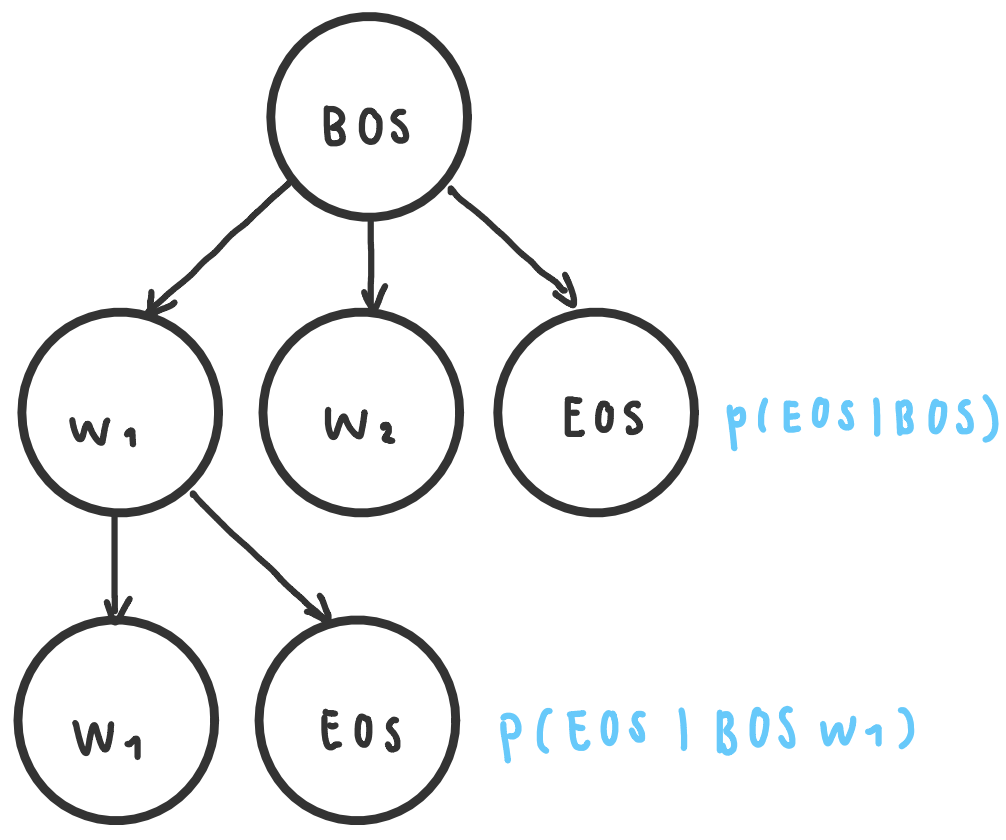
\includegraphics[height=10mm]{inhalt/images/NLP/06_language_models_1.png}
\end{multicols}